%%
%% This is file `./samples/shortsample.tex',
%% generated with the docstrip utility.
%%
%% The original source files were:
%%
%% apa6.dtx  (with options: `shortsample')
%% ----------------------------------------------------------------------
%% 
%% apa6 - A LaTeX class for formatting documents in compliance with the
%% American Psychological Association's Publication Manual, 6th edition
%% 
%% Copyright (C) 2011-2017 by Brian D. Beitzel <brian at beitzel.com>
%% 
%% This work may be distributed and/or modified under the
%% conditions of the LaTeX Project Public License (LPPL), either
%% version 1.3c of this license or (at your option) any later
%% version.  The latest version of this license is in the file:
%% 
%% http://www.latex-project.org/lppl.txt
%% 
%% Users may freely modify these files without permission, as long as the
%% copyright line and this statement are maintained intact.
%% 
%% This work is not endorsed by, affiliated with, or probably even known
%% by, the American Psychological Association.
%% 
%% ----------------------------------------------------------------------
%% 
\documentclass[jou]{apa6}

\usepackage[american]{babel}

\usepackage{csquotes}
\usepackage[style=apa,sortcites=true,sorting=nyt,backend=biber]{biblatex}
\DeclareLanguageMapping{american}{american-apa}
\addbibresource{bibliography.bib}


%%%%%%%%%%%%%%%%%%%%%%%%%%%%%%%%%%%%%%%%
%% Discrete Structures
%% The start of RBS stuff
%%%%%%%%%%%%%%%%%%%%%%%%%%%%%%%%%%%%%%%%

% Working internal and external links in PDF
\usepackage{hyperref}
% Extra math symbols in LaTeX
\usepackage{amsmath}
\usepackage{gensymb}
\usepackage{amssymb}
% Enumerations with (a), (b), etc.
\usepackage{enumerate}

\let\OLDitemize\itemize
\renewcommand\itemize{\OLDitemize\addtolength{\itemsep}{-6pt}}

\usepackage{etoolbox}
\makeatletter
\preto{\@verbatim}{\topsep=3pt \partopsep=3pt }
\makeatother

% These sizes redefine APA for A4 paper size
\oddsidemargin 0.0in
\evensidemargin 0.0in
\textwidth 6.27in
\headheight 1.0in
\topmargin -24pt
\headheight 12pt
\headsep 12pt
\textheight 9.19in



\title{Quiz for Week02}
\author{Discrete Structures, Fall 2020}
\affiliation{RBS}

\leftheader{Discrete Structures (W2): Quiz}

\abstract{%
}

%\keywords{}

\begin{document}
%\maketitle

\twocolumn
{\Large Discrete Structures (W2): Quiz}

\thispagestyle{empty}

\vspace{6pt}
{\bf Question 1.} Let $p \in \mathbb{Z}^{+}$ be a positive integer.
Translate into predicate logic: ``$p$ is a prime number.'' (Prime numbers
have exactly two positive divisors: $1$ and the number itself).\\
{\em Note.} Use ``infix'' notation in your expressions: write 
$a\,\mid\,b$ whenever $a$ divides $b$; write $x < y$, if $x$ is less than $y$.\\
{\scriptsize \em (Write predicate expression; specify domains for quantifiers.)}\\
\framebox(220,30){}

% box for an answer

{\bf Question 2.} We define $P(n)$ to be true
iff $n$ is a prime. For example, 
$P(2)$, $P(3)$, $P(5)$ etc.\ are true,
but $P(1)$, $P(4)$ etc.\ are all false.\\
Translate into predicate logic: ``There are arbitrarily large primes'', i.e.\ there is no 
such thing as the largest prime.
(Use just the $P(n)$ and inequaly symbols as predicates.)\\
{\scriptsize \em (Write predicate expression; specify domains for quantifiers.)}\\
\framebox(220,30){}


{\bf Question 3.} You can express the exclusive OR as a {\em disjunction of conjunctions}:
\begin{center}
$a \oplus b \;\equiv\; (a \wedge \neg b) \vee (\neg a \wedge b)$.
\end{center}
Indeed, for $a \oplus b$ to be true, you should 
either have $a$ true and $b$ false: $(a \wedge \neg b)$ or 
$a$ false and $b$ true: $(\neg a \wedge b)$. 
Express this truth table as a {\em disjunction of conjunctions} as well \textendash{}
list all cases when it takes value {\tt T}:

\begin{tabular}{ c | c | c | c }
$p$ & $q$ & $r$ & $E(p,q,r)$ \\ \hline
{\tt T} & {\tt T} & {\tt T} & {\tt T} \\ \hline
{\tt T} & {\tt T} & {\tt F} & {\tt F} \\ \hline
{\tt T} & {\tt F} & {\tt T} & {\tt F} \\ \hline
{\tt T} & {\tt F} & {\tt F} & {\tt F} \\ \hline
{\tt F} & {\tt T} & {\tt T} & {\tt F} \\ \hline
{\tt F} & {\tt T} & {\tt F} & {\tt T} \\ \hline
{\tt F} & {\tt F} & {\tt T} & {\tt F} \\ \hline
{\tt F} & {\tt F} & {\tt F} & {\tt T} \\ \hline
\end{tabular}\\
{\scriptsize \em (Write Boolean expression as disjunction of conjunctions)}\\
\framebox(220,30){}


{\bf Question 4.} There are altogether $10$ children: $\{ c_1,\ldots,c_{10} \}$ and 
$10$ hats: $\{ h_1,\ldots,h_{10} \}$. Initially, every child $c_i$ has his own hat $h_i$.
When they were about to leave a party, there was an electricity 
blackout, and they grabbed hats at random (not necessarily their own). 
Predicate $G(i,j)$ is true iff child $c_i$ grabbed hat $h_j$.\\
{\bf (a)} Write the domain set and the range set of the 
predicate function $G$.\\
\framebox(220,20){}\\
{\bf (b)} Translate this statement into predicate logic: ``Nobody grabbed his/her own hat.''\\
\framebox(220,30){}


{\bf Question 5.} Translate these two sequences into predicate logic:\\
{\bf (a)} In the interval of real numbers $(0;1)$ there is no smallest number.\\
{\scriptsize \em (Write predicate expression; specify domains for quantifiers)}\\
\framebox(220,30){}\\
{\bf (b)} For the function $f(x) = x^2 - x$ defined on $(0;1)$ there exists the smallest value.\\
{\scriptsize \em (Write predicate expression; specify domains for quantifiers)}\\
\framebox(220,30){}


{\bf Question 6.} Predicates $\mathrm{Plane}(x,y)$, 
$\mathrm{Rail}(x,y)$ show how to travel between cities $A,B,C$. 

\vspace{-10pt}
\begin{center}
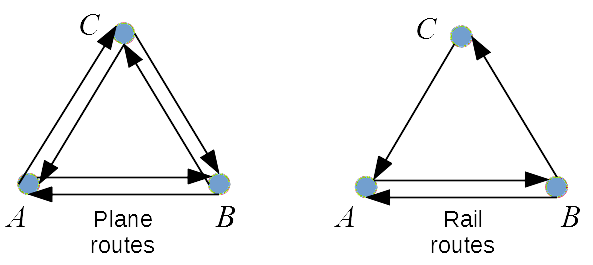
\includegraphics[width=2.5in]{relation-graphs.png}
%{\em Figure 1: Diagrams with Transport Links.}
\end{center}
\vspace{-10pt}
They have these following truth tables:
\begin{center}
\begin{tabular}{c|ccc}
Plane & $A$ & $B$ & $C$ \\ \hline
$A$ & $\mathtt{F}$ & $\mathtt{T}$ & $\mathtt{T}$ \\
$B$ & $\mathtt{T}$ & $\mathtt{F}$ & $\mathtt{T}$ \\
$C$ & $\mathtt{T}$ & $\mathtt{T}$ & $\mathtt{F}$
\end{tabular}
\hspace{2ex}
\begin{tabular}{c|ccc}
Rail & $A$ & $B$ & $C$ \\ \hline
$A$ & $\mathtt{F}$ & $\mathtt{T}$ & $\mathtt{F}$ \\
$B$ & $\mathtt{T}$ & $\mathtt{F}$ & $\mathtt{T}$ \\
$C$ & $\mathtt{T}$ & $\mathtt{F}$ & $\mathtt{F}$
\end{tabular}
\end{center}
Find the truth values of these statements:\\
{\bf (a)} $\forall x \exists y, \neg \mathrm{Plane}(x,y)$\\
{\bf (b)} $\forall x \forall y \exists z, \mathrm{Plane}(x,z) \wedge \mathrm{Plane}(z,y)$\\
{\bf (c)} $\exists x \exists y \exists z, \mathrm{Rail}(x,y) \wedge \mathrm{Rail}(y,z) \wedge \mathrm{Rail}(z,x)$\\
{\bf (d)} $\forall x \forall y \exists z, \mathrm{Rail}(x,z) \wedge \mathrm{Rail}(z,y)$\\
{\em Note.} In the truth tables the first argument is
represented by row, the second is represented by column. 
For example, $\mathrm{Rail}(\mathtt{C}, \mathtt{B}) = \mathtt{F}$ (3rd row,
2nd column).



{\bf Question 7.} 
Two positive real numbers $x,y \in \mathbb{R}^{+}$ are given. 
Translate into predicate logic this statement:
``Values $x$ and $y$ are the same, if we round them to two 
decimal places.'' Use variable names, arithmetic operations and 
the floor function ($\lfloor x \rfloor$ is the largest integer not
exceeding $x$).\\
{\em Note.} Rounding $x$ to two decimal places finds the 
number $\frac{p}{100}$ closest to $x$. 
If two are equally close, then round up.
(For example, $3.14159$ rounds to $3.14$; $3.144999$ rounds to $3.14$, 
but $3.145$ rounds to $3.15$.)\\
{\scriptsize \em (Write predicate expression; specify domains for quantifiers)}\\
\framebox(220,30){}

\newpage

\section{Answers}

{\bf Question 1:} Answer: Number $n \in \mathbb{Z}^{+}$ is a {\em prime} iff
\begin{align}
P(n) & :=\, \forall d \in \mathbb{Z}^{+}, \nonumber \\
 & \left( n > 1 \wedge \left( d \,\mid\, n \;\rightarrow\; (d = 1 \vee d = n) \right)\right). \nonumber
\end{align}
It is essential to require that $d$ is positive: $d \in \mathbb{Z}^{+}$, since prime numbers
may have negative divisors, say $n=7$ is divisible by four numbers: $d=-7, -1, 1, 7$. It is 
simpler to deal with only positive $d$ such that $d\,\mid\,n$.\\
Also it is essential that $n>1$; otherwise $n=1$ would also turn out to be a prime. Which is wrong, since it 
only has one divisor, not {\bf exactly} two.

\vspace{10pt}
{\bf Question 2:} Answer:\\[5pt]
\framebox(220,20){
$\forall N \in \mathbb{Z}^{+}\; \exists p \in \mathbb{Z}^{+},\;\left( p > N \,\wedge\, P(p) \right).$
}
In the predicate language this is a statement that for any (arbitrarily large) positive integer $N$ 
there exists an even larger positive integer $p$ such that $p$ is a prime. 

\vspace{10pt}
{\bf Question 3:} Answer:\\[5pt]
\framebox(220,20){
$(p \wedge q \wedge r) \vee (\neg p \wedge q \wedge \neg r) \vee (\neg p \wedge \neg q \wedge \neg r).$
}
For each row, where the truth table has value ${\tt T}$, we write one more
subexpression. Since there are just $3$ such rows in the table, 
there should be a disjunction $(\ldots) \vee (\ldots) \vee (\ldots)$. 
For example, the 2nd term $(\ldots)$ corresponds to the case, where $p = \mathtt{F}$, 
$q = \mathtt{T}$, $r = \mathtt{F}$, so we write $(\neg p \wedge q \wedge \neg r)$ (and other cases
are treated similarly).

\vspace{10pt}
{\bf Question 4:} {\bf (a)} Answer:\\[5pt]
\framebox(220,20){
$G\,:\, \{ 1,\ldots,10\} \times \{ 1,\ldots,10\} 
\,\rightarrow\, \{ \mathtt{T}, \mathtt{F} \}$.
}
Note that the predicate $G(i,j)$ acts not on the sets of children and hats, but 
on their {\em numbers}. Both $i$ and $j$ change over the same set $\{ 1,\ldots,10\}$.\\
{\bf (b)} Answer:\\[5pt]
\framebox(220,20){
$\forall i \in \{ 1,\ldots,10\}\; \forall j \in \{ 1,\ldots,10\},\; \,\left( G(i,j) \rightarrow i \neq j \right).$
}
{\em Note.} From the problem statement, some other predicate logic statements follow.
For example, we could also write another predicate logic statement saying that no child 
grabbed more than $1$ hat and every hat was taken. It is not wrong to add such clauses, 
but there were not part of the requirement of the problem, so the above answer is the 
simplest possible.

\vspace{10pt}
{\bf Question 5:} 
{\bf (a)} In the interval of real numbers $(0;1)$ there is no smallest number:\\[5pt]
\framebox(220,20){
$\forall x_1 \in (0;1)\, \exists x_2 \in (0;1),\, \left( x_2 < x_1 \right)$.
}\\
In this example the domain is $(0;1)$. It has no smallest number, since for every positive $x_1 > 0$
there exists an even smaller positive number. For example, we can take $x_2 = x_1/2$.\\
{\bf (b)} For the function $f(x) = x^2 - x$ defined on $(0;1)$ there exists the smallest value.\\[5pt]
\framebox(220,20){
$\exists x_0 \in (0;1)\,\forall x \in (0;1),\,\left( f(x) \geq f(x_0) \right)$.
}
In this case $f(x_0)$ is the smallest value, which is reached for the argument $x_0$. 
By the way, in our specific case this predicate logic statement is true. 
We can take $x_0 = \frac{1}{2} \in (0;1)$. This value gives the smallest value to 
the quadratic function $f(x) = x^2 - x$. But predicate logic statement can be written for 
any function $f(x): (0;1)\rightarrow \mathbb{R}$: 
If it does not have the minimum on $(0;1)$, the statement would be false.


\vspace{10pt}
{\bf Question 6:} Answers:\\
{\bf (a)} $\forall x \exists y, \neg \mathrm{Plane}(x,y) = \mathtt{True}$.\\
Indeed, for each city $x$ there is a city $y$ such that there is no plane connection. You can take $x = y$ (no 
plane goes from $x = A$ $x=B$, or $x=C$ to itself).\\
{\bf (b)} $\forall x \forall y \exists z, \mathrm{Plane}(x,z) \wedge \mathrm{Plane}(z,y)  = \mathtt{True}$.\\
Reasoning with $3$ variables and truth tables is not too convenient, but we can reason in plain English:
Is it true that for every two cities $x$ and $y$ (possibly $x = y$), there exists a city $z$, so that
one can fly from $x$ to $y$ via $z$? This is true and visible from the triangle graph.\\
{\bf (c)} $\exists x \exists y \exists z, \mathrm{Rail}(x,y) \wedge \mathrm{Rail}(y,z) \wedge \mathrm{Rail}(z,x) = \mathtt{True}$.\\
There exists a circular trip with rail. For example, we can take $(x,y,z) = (A,B,C)$. Then we can go from $A$ to $B$, 
$B$ to $C$ and $C$ to $A$.\\
{\bf (d)} $\forall x \forall y \exists z, \mathrm{Rail}(x,z) \wedge \mathrm{Rail}(z,y)= \mathtt{False}$.\\
If we take cities $x = A$ and $x = B$, then there exists no two-leg trip from $A$ to $B$ going through some city $z$.\\

\vspace{10pt}
{\bf Question 7:} Answer:\\[5pt]
\framebox(220,30){
${\displaystyle \left\lfloor 100x + \frac{1}{2} \right\rfloor = \left\lfloor 100y + \frac{1}{2} \right\rfloor}$. 
}
The fact that two numbers (for example, expressing money) round to exactly the same number
of euros and eurocents, can be written without any quantifiers. It is a predicate:
$P(x,y)$, with $P\,:\,\mathbb{R}^{+} \times \mathbb{R}^{+} \rightarrow \{ \mathtt{T},\mathtt{F} \}$.\\
{\em Note.} We could also write this with quantifiers. For example:
for the given $x,y$ there exists a non-negative integer number $z \in \mathbb{Z}^{0+}$ ($z$ expresses 
the number of eurocents) such that both $\left| 100x - z \right| \leq 0.5$ and $\left| 100y - z \right| \leq 0.5$. 
But writing such an expression would be longer, since we need to sort out the special case, when 
exactly one half of a eurocent ($x = 0.005$) is rounded up.










\end{document}



%%%%%%%%%%%%%%%%%%%%%%%%%%%%%%%%%%%%%%%%
%% End of RBS stuff
%%%%%%%%%%%%%%%%%%%%%%%%%%%%%%%%%%%%%%%%


%% 
%% Copyright (C) 2011-2017 by Brian D. Beitzel <brian at beitzel.com>
%% 
%% This work may be distributed and/or modified under the
%% conditions of the LaTeX Project Public License (LPPL), either
%% version 1.3c of this license or (at your option) any later
%% version.  The latest version of this license is in the file:
%% 
%% http://www.latex-project.org/lppl.txt
%% 
%% Users may freely modify these files without permission, as long as the
%% copyright line and this statement are maintained intact.
%% 
%% This work is not endorsed by, affiliated with, or probably even known
%% by, the American Psychological Association.
%% 
%% 
%% This work is "maintained" (as per LPPL maintenance status) by
%% Brian D. Beitzel.
%% 
%% This work consists of the file  apa6.dtx
%% and the derived files           apa6.ins,
%%                                 apa6.cls,
%%                                 apa6.pdf,
%%                                 README,
%%                                 APAamerican.txt,
%%                                 APAbritish.txt,
%%                                 APAdutch.txt,
%%                                 APAenglish.txt,
%%                                 APAgerman.txt,
%%                                 APAngerman.txt,
%%                                 APAgreek.txt,
%%                                 APAczech.txt,
%%                                 APAturkish.txt,
%%                                 APAendfloat.cfg,
%%                                 apa6.ptex,
%%                                 TeX2WordForapa6.bas,
%%                                 Figure1.pdf,
%%                                 shortsample.tex,
%%                                 longsample.tex, and
%%                                 bibliography.bib.
%% 
%%
%% End of file `./samples/shortsample.tex'.
